\chapter{Introduction}

\section{General Overview of the Problem}

Perception has always been a fundamental task in the field of robotics. In order to perform actions and modify its environment in an automated manner, a robot must be provided with proper knowledge of its surroundings via sensor data, and appropriate processing of this data.

\begin{figure}[ht]
    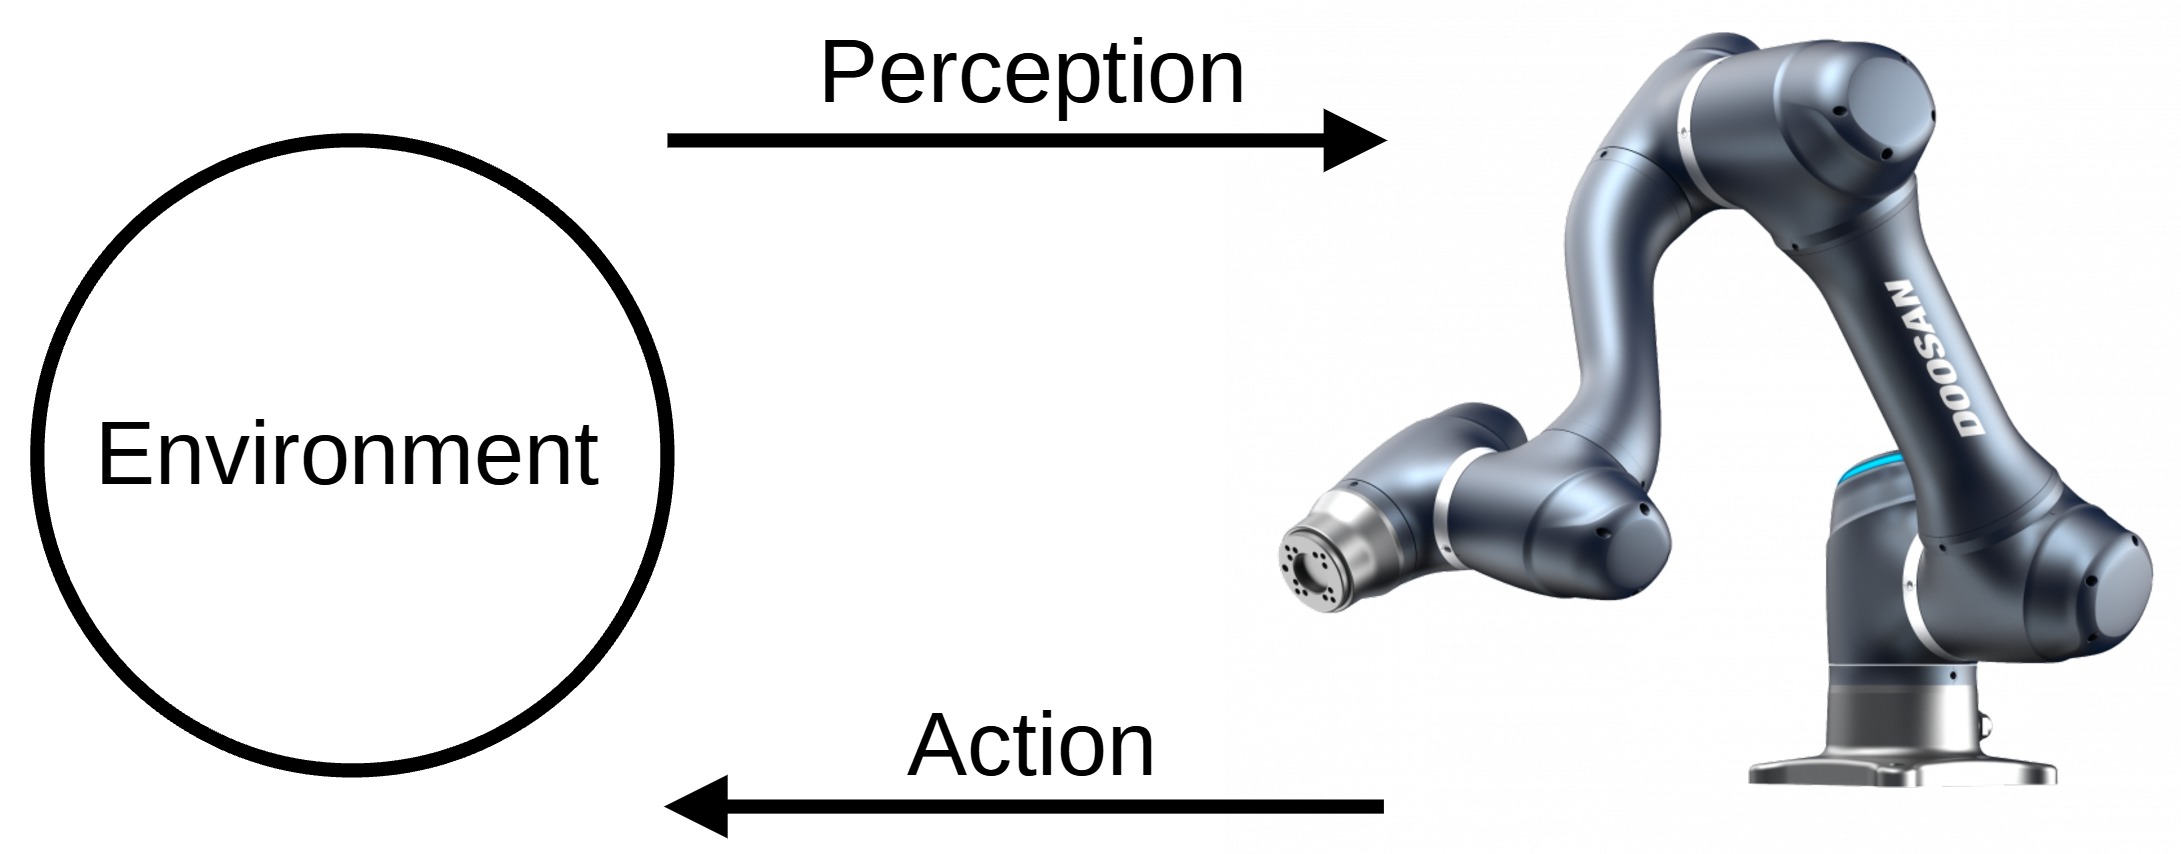
\includegraphics[width=0.75\textwidth]{perception_action.png}
    \caption{The main ways a robot interacts with the environment: perception and action.}
\end{figure}

One of the most readily available, and at the same time inherently complex sensors applicable to such a scenario is the color camera. While commonly used sensors, such as thermometers or encoders, usually output a single value that represents the physical quantity they are measuring, cameras generate data on an entirely different scale: a relatively low resolution 1280x720 pixel RGB sensor outputs an array of 2'774'800 values, thirty to sixty times per second. Furthermore, these values do not directly reflect any physical quantities, but must be further processed to extract the necessary measurments. This limits the viability of cameras in real-time control applications.

Neural networks, however, are perfectly suited to face these challenges. They are built to work with a large number of inputs in parallel, and are capable of modelling complex functions through proper training. In particular, Convolutional Neural Networks (CNNs) have been widely applied to the field of image processing, due to their independance from prior knowledge, the relatively little amount of pre-processing they require, and a decreased subsceptibility to overfitting when compared to their fully-connected counterparts.

\begin{figure}[ht]
    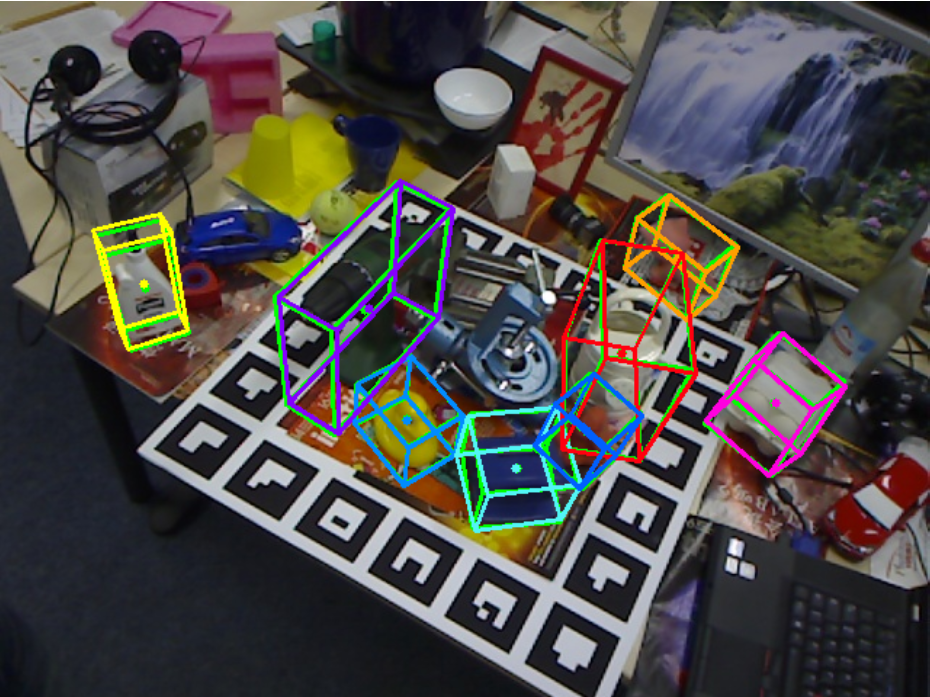
\includegraphics[width=0.6\textwidth]{efficientpose_example.png}
    \caption{Multi-object inference on an image from the LINEMOD\cite{linemod} dataset performed by EfficientPose\cite{bukschat2020efficientpose}, a 6D pose estimation CNN. Green bounding boxes visualize ground truth poses while other colors represent estimations.} 
\end{figure}

Two particular subfields of image processing that have advanced by leaps and bounds in recent years are object identification and pose estimation. Object identification tackles the problem of verifying whether an image contains a particular object, and in which part of the image, while pose estimation techniques provide the position and orientation of the detected object in relation to the camera. Both of these tasks greatly benefit from CNNs, and are very relevant to robotics applications.

\section{Thesis Goals}

Our objective in this thesis is therefore to verify the applicability and performance of a state-of-the-art 6D pose estimation CNN to a robotics scenario, and the difficulties involved in doing so. When working with machine learning approaches, one faces two main issues:
\begin{itemize}
    \item The necessity of acquiring large amounts of data to train the network.
    \item The opaqueness of the resulting network to conventional analysis.
\end{itemize}
These two issues are deeply interconnected: neural networks are incapable of understanding cause and effect relationships, being only practiced in percieving and optimizing the relationship between input and output data. Therefore the only way to change their behaviour is to modify their \emph{training inputs}, and associated desired outputs (the \emph{ground truth}), which together form a \emph{dataset}.

However, acquiring the necessary data to build a high-quality dataset is often time-consuming and expenisve. Our initial goal is therefore to improve the applicability of machine learning approaches to pose estimation tasks by facilitating this process. For this purpose, we demonstrate an approach for quickly and easily generating large amounts of synthetic labelled data starting from a set of background images, providing realistic depictions of a small number of objects of interest in a determined environment.

\begin{figure}[ht]
    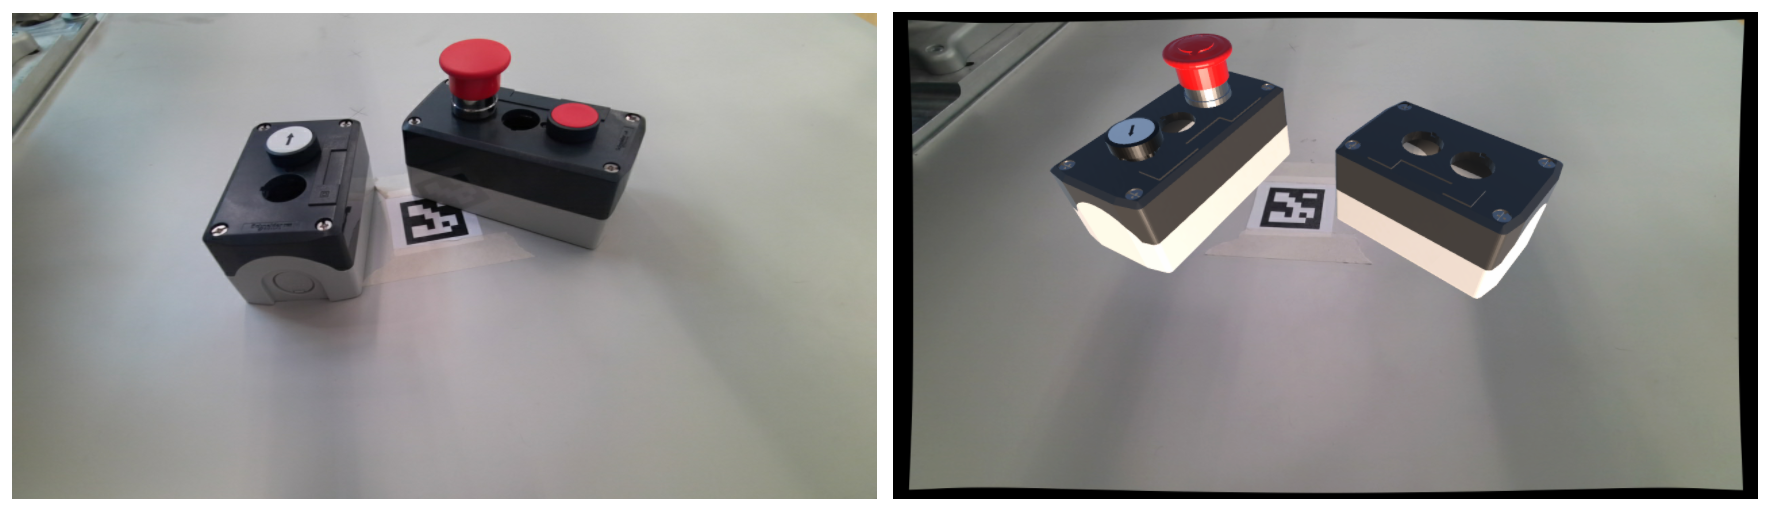
\includegraphics[width=0.9\textwidth]{real_vs_simulated.png}
    \caption{Side-by-side comparison of a real image and a generated training image resulting from our pipeline.}
\end{figure}

We then verify the performance of a model trained on this data, and whether it is capable of effectively generalising to real world conditions.

For many applications in industrial and collaborative robotics, estimations of the pose by themselves may not be sufficient to complete a task, but more high-level knowledge of the semantic state of a scene is required. Therefore we developed a method that uses the outputs from a pose estimation network to compute the overall semantic state of a scene, and tested its reliability in a simple assembly scenario.

Finally, by combining the results of the previous two methods, we verified the performance of the complete system in a real-world application by using a the estimations from the trained network and from our semantic meaning extractions algorithm to plan the movement of a robotic manipulator. 

\section{Achieved Results}

Our dataset generation provided to be crucial when testing out different variations of traning inputs and their effect on the final performance of the network. Overall, the complete system was able to generalise in a satisfactory manner to real-world conditions. However, its performance may not be sufficient for tasks that require very high precision to be completed, and is highly dependant on the performance of the underlying neural network.

\section{Thesis structure}
The rest of this thesis is organized as follows.  We will begin by examining the current state-of-the-art for pose estimation approaches (chapter 2), and we will give some background on the pose estimation network we chose as the basis of our approach, EfficientPose (chapter 3). We will then go over our methodologies and underlying motivations (chapter 4), and the metrics and experiments used to evaluate them (chapter 5). Finally, we will lay out the results of our experiments (chapter 6), and conclude the thesis (chapter 7).
